\chapter{Algorithmen zur Phasenrückgewinnung}
\label{chap:anhang_algos}
Die grundlegende Iteration der iterativen Rekonstruktionsalgorithmen ER, HIO und RAAR in ihrer Projektionsschreibweise sind in \Fref{tab:ipr} dargestellt.

Aus Gründen der Simplizität wird davon ausgegangen, dass die Realraumbeschränkungen nur den Support beinhalten, d.h. der Realraum-Projektor $P_s$ geschrieben werden kann als 
\begin{align}
	P_s\rho (x)=\begin{cases}
	\rho (x)  &\text{für } x\in S\\
	\mathbb{0}  &\text{für }x\notin S
	\end{cases} &   &   
	P_{\bar{s}}\rho (x)=\begin{cases}
	\mathbb{0} &\text{für } x\in S\\
	\rho (x)   &\text{für }x\notin S
	\end{cases}
\end{align}
und somit als reiner Support-Projektor aufgefasst werden kann. In der Literatur wird unter der Bezeichnung $P_s$ teilweise auch ein Projektor bezeichnet der außerdem weitere Forderungen im Realraum beinhaltet. Im Rahmen dieser Arbeit nur für den ER-Algorithmus zusätzlich eine Form implementiert, deren Realraum-Projektor eine reele, positive Lösung erzwingt (\texttt{reconstruction/ERiterRealPos.m}), da das mittelfristige Ziel die Rekonstruktion der Austrittswelle inklusive der relativen Phasenbeziehungen darstellt.
 
Für den HIO-Algorithmus gilt mit jenem $P_s$ 
\begin{align*}
	\begin{rcases}	
	P_m\rho_n                               & \text{für } x\in S    \\
	\left[\mathbb{1}-\beta P_m\right]\rho_n & \text{für } x\notin S 
	\end{rcases}	
	=\left[P_sP_m+\left(P_{\bar{s}}-\beta P_{\bar{s}} P_m\right)\right]\rho_n
	\,.
\end{align*}
Diese Form erleichtert das Verständnis von \fref{fig:recon}. Zum weiteren Verständnis ist in \fref{fig:raar} der Prozess für den RAAR-Algorithmus schrittweise dargestellt.
	
Die implementierte Form des RAAR Algorithmus' basiert auf folgender Umformung:
\begin{align*}
	\frac{\beta}{2}\left(R_sR_m+\mathbb{1}\right)
	                              & =\frac{\beta}{2}\left((2P_s-\mathbb{1})(2P_m-\mathbb{1})+\mathbb{1}\right) 
	=2\beta P_sP_m-\beta P_s-\beta P_m+\beta\mathbb{1}\\
	\frac{\beta}{2}\left(R_sR_m+\mathbb{1}\right)+\left(1-\beta\right) P_m
	                              & =2\beta P_sP_m+\beta (\mathbb{1}-P_s)+ (1-2\beta)P_m                       \\
	                              & =                                                                          
	\begin{cases}
	P_m                           & \text{für } r\in S                                                        \\
	(1-2\beta)P_m+\beta\mathbb{1} & \text{für } r\notin S                                                     
	\end{cases}\\
\end{align*}
\begin{table}
	\centering
	\begin{tabular}{cc}
		\hline\hline
		Algorithmus                             & $\rho_{n+1}$                                                                               \\ 							
		\hline
		ER                                      & $P_sP_m\rho_n$                                                                             \\ 								
		HIO                                     & $\begin{cases}                                                                             
		P_m\rho_n                               & \text{für } x\in S                                                                        \\
		\left[\mathbb{1}-\beta P_m\right]\rho_n & \text{für } x\notin S                                                                     
		\end{cases}$\\
		RAAR                                    & $\left[\frac{\beta}{2}\left(R_sR_m+\mathbb{1}\right)+\left(1-\beta\right)P_m\right]\rho_n$ \\																
		\hline\hline
	\end{tabular}
	\caption[IPR-Algorithmen]{Iterationsschritte der implementierten IPR-Algorithmen.}
	\label{tab:ipr}
\end{table}	

\begin{figure}
	\centering
	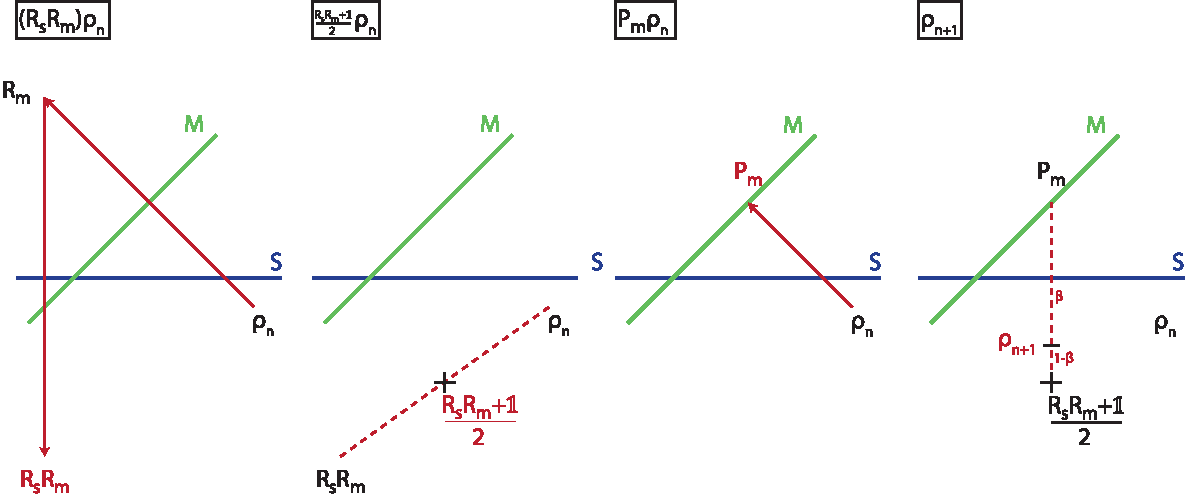
\includegraphics[width=1\textwidth]{images/raar.pdf}
	\caption[RAAR]{Detailierte Darstellung von \fref{fig:recon} für RAAR, von links nach rechts: 1. Die Anwendung des Modulus-Reflektors gefolgt vom Support-Reflektor liefert $R_sR_m\rho$. 2. Der Mittelpunkt von $R_sR_m\rho$ und $\rho$ ist $(\sfrac{1}{2}R_sR_m+\mathbb{1})\rho$. 3. Anwenden des Modulus-Projektors liefert $P_m\rho$. 4. Die Kombination von $P_m\rho$ und $(\sfrac{1}{2}R_sR_m+\mathbb{1})\rho$ im Verhältnis $\beta$ und $1-\beta$ liefert das Ergebnis der Iteration  und somit den Startpunkt für die nächste Iteration ($\rho_{n+1}$).}
	\label{fig:raar}
\end{figure} 	
